\documentclass[conference]{IEEEtran}
\usepackage{cite}
\usepackage{amsmath,amssymb,amsfonts}
\usepackage{graphicx}
\usepackage{booktabs}
\usepackage{multirow}
\usepackage{xcolor}
\usepackage{url}
\usepackage{hyperref}
\hypersetup{colorlinks=true,linkcolor=blue,citecolor=blue,urlcolor=blue}

\begin{document}
\setlength{\textfloatsep}{6pt plus 1pt minus 1pt}
\setlength{\floatsep}{6pt plus 1pt minus 1pt}
\setlength{\dbltextfloatsep}{6pt plus 1pt minus 1pt}
\setlength{\dblfloatsep}{6pt plus 1pt minus 1pt}

\title{Selective Test-Time Adaptation and Fail-Closed Safeguards for Digital Pathology: Multicenter Classification and Dense Detection Under Domain Shift}

\author{
\IEEEauthorblockN{Anonymous Authors}
\IEEEauthorblockA{Paper under double-blind scientific review}
}

\maketitle

\begin{abstract}
Deep learning models trained on source pathology centers frequently degrade when deployed across unseen hospitals and optical scanners.
Test-time adaptation (TTA) aims to mitigate distribution shift using unlabeled target data, but unconstrained entropy minimization is unstable: under a fair BatchNorm-affine protocol on Camelyon17-WILDS patch metastasis classification, Tent collapses on 2 of 5 random seeds ($F_1 \approx 0.05$).
We investigate \textbf{selective} TTA and \textbf{fail-closed safeguards} across two distinct histopathology tasks: binary metastasis classification and dense mitotic figure detection.
For patch classification on Camelyon17-WILDS (ResNet-18, target Hospital~2, $N=85{,}054$ patches across 10 whole-slide images), a hard uncertainty gate admits target patches to adaptation only when predictive uncertainty falls below a threshold $\tau$ fixed on a held-out center.
Across five random seeds, selective gating reduces the harmful adaptation rate from $0.187 \pm 0.179$ (Tent) to $0.007 \pm 0.003$ ($>25\times$ reduction) and improves $F_1$ score on every seed ($+0.023$ vs.\ frozen source, 95\% CI $[0.010, 0.036]$).
However, Monte Carlo Dropout variance (UTTA-Med) achieves similar observed performance to softmax confidence gating ($p=0.869$), and AUROC gains are not statistically significant ($+0.006$, 95\% CI $[-0.012, +0.024]$).
For dense mitotic figure detection on held-out MIDOG 2021 Scanner~3 (Faster R-CNN, 50 cases, 1,100 spatially stratified patches, 3 seeds), we evaluate SafeAdapt---a controller combining source-anchored admission gating, atomic rollback, and permanent source fallback.
SafeAdapt achieves the same mean $F_1$ score as the frozen source detector ($0.4774$), yielding an observed seed-macro $F_1$ difference of $0.0000$ (all 10,000 paired case-clustered bootstrap replicates equal $0.0000$).
Early silence alarms triggered permanent source fallback in all three seeds (Seed 42 at patch 102; Seed 7 at patch 80; Seed 123 at patch 58), preserving source performance rather than achieving positive target adaptation.
Conventional TTA and monitored TTA without permanent fallback exhibit mean $F_1$ differences of $-0.0072$ and $-0.0065$, respectively, with bootstrap confidence intervals spanning zero ($[-0.0417, +0.0255]$ and $[-0.0412, +0.0262]$).
These findings demonstrate that selective gating and circuit-breaker fallbacks contain failure and prevent catastrophic collapse under domain shift, but operational failure containment does not equate to positive adaptation gain or clinical validation.
\end{abstract}

\begin{IEEEkeywords}
Test-time adaptation, uncertainty estimation, digital pathology, fail-closed safeguards, Camelyon17, MIDOG 2021, domain shift, reliability.
\end{IEEEkeywords}

\section{Introduction}
Cross-center distribution shift is an unavoidable challenge in clinical computational pathology: variations in whole-slide scanner optics, sensor calibration, staining protocols, microtomy, and patient populations induce substantial domain divergence~\cite{koh2021wilds,bandi2018camelyon17,aubreville2023mitosis}.
A model trained to high accuracy on source hospitals can retain strong in-domain ranking while suffering severe drops in sensitivity, calibration, and diagnostic precision upon deployment at an unseen institution.

Test-time adaptation (TTA) addresses this gap by updating a model's parameters using unlabeled batches from the target domain at inference time~\cite{wang2021tent,liang2023comprehensive}.
Unsupervised entropy minimization (Tent)~\cite{wang2021tent} has become a standard baseline because of its architectural simplicity.
However, entropy minimization operates under an implicit assumption: that the model's low-entropy predictions on out-of-domain samples are largely correct.
When distribution shift violates this premise, high-confidence erroneous pseudo-labels act as reinforcement signals, creating a self-reinforcing feedback loop that rapidly destabilizes model representations~\cite{histopathc2026}.

This paper presents a systematic \textbf{reliability and failure-containment study} across two operational regimes in digital pathology:
\begin{enumerate}
\item \textbf{Multicenter Metastasis Classification:} High-throughput binary patch classification on Camelyon17-WILDS~\cite{koh2021wilds}, where dense tissue morphology is evaluated across five clinical centers.
\item \textbf{Dense Mitotic Figure Detection:} Spatially sparse object detection on MIDOG 2021~\cite{aubreville2023mitosis}, where rare cellular divisions (mitoses) must be localized across diverse slide-scanning hardware.
\end{enumerate}

We test a precise operational hypothesis: \emph{can selective uncertainty gating and fail-closed monitoring contain TTA failure modes without inducing negative adaptation?}

\textbf{Contributions.}
\begin{enumerate}
\item \textbf{Leakage-Controlled Multicenter Protocol:} We define a strict evaluation protocol on Camelyon17-WILDS where source models are trained on hospitals $\{0,3,4\}$, adaptation hyperparameters ($\tau$) are selected exclusively on held-out validation hospital $\{1\}$, and adaptation is evaluated on unseen hospital $\{2\}$ ($85{,}054$ patches across 10 whole-slide images) over five random seeds.
\item \textbf{Selective Gating Evaluation:} Across five seeds, we demonstrate that hard uncertainty gating prevents Tent collapse, reduces the harmful adaptation rate from $0.187 \pm 0.179$ to $0.007 \pm 0.003$ ($>25\times$), and improves $F_1$ on every seed ($+0.023$, 95\% CI $[0.010, 0.036]$). We show that Monte Carlo Dropout variance (UTTA-Med) and softmax confidence gating achieve similar observed performance in binary classification ($p=0.869$).
\item \textbf{Exploratory Multi-Scanner Detection Evaluation:} On held-out MIDOG 2021 Scanner~3 (50 cases, 1,100 spatially stratified patches in a 4x4 grid), we evaluate five adaptation arms across three pretrained detector seeds. SafeAdapt achieves a mean $F_1$ score identical to the frozen source baseline ($0.4774$, observed $\Delta F_1 = 0.0000$, 95\% bootstrap CI $[0.0000, 0.0000]$) because early detection-silence alarms triggered permanent source fallback across all three seeds.
\item \textbf{Forensic Provenance \& Methodological Disclosures:} We distinguish between accuracy improvement, failure containment through fallback, statistical uncertainty, computational correctness, and clinical validation. We document the post-halt tissue threshold amendment, runner versioning, and adaptation implementation differences between experimental stages.
\end{enumerate}

We make \textbf{no claim} of a new state-of-the-art AUROC, nor do we claim clinical equivalence or statistical superiority for SafeAdapt on dense detection.
The verifiable finding is that selective gating and circuit-breaker fallbacks contain catastrophic divergence under real distribution shift, operating as essential safety mechanisms rather than performance enhancers.

\section{Related Work}
\textbf{Test-Time Adaptation.}
Tent updates BatchNorm affine parameters ($\gamma, \beta$) via prediction entropy minimization~\cite{wang2021tent}.
EATA adds an entropy threshold to exclude high-entropy samples and incorporates a Fisher-regularized anti-forgetting objective~\cite{niu2022eata}.
SAR stabilizes adaptation using sharpness-aware minimization while filtering high-entropy samples~\cite{niu2023sar}.
While EATA and SAR employ point-estimate entropy, UTTA-Med uses stochastic predictive variance derived from Monte Carlo Dropout~\cite{gal2016dropout}.
We evaluate these approaches under an identical BatchNorm-affine, frozen-running-statistics, single-pass protocol to eliminate parameter scope as an experimental confound.

\textbf{Medical TTA \& Digital Pathology Benchmarks.}
In medical imaging, CertainTTA integrates predictive and epistemic uncertainty for segmentation adaptation~\cite{certaintta2025}.
UAD-FM investigates causal adaptation and calibration with pathology foundation models~\cite{uadfm2025}.
TT-SaD performs diffusion-based stain normalization for patch classification~\cite{ttsad2024}.
SicTTA selects source-friendly samples for continual segmentation~\cite{sictta2026}, and MedSeg-TTA benchmarks segmentation methods across seven imaging modalities~\cite{yu2025medsegtta}.
AETTA estimates test-time accuracy using dropout disagreement~\cite{lee2024aetta}.
Recent benchmarking by Bahumanya et al.~\cite{bahumanya2026explanationstability} highlights that feature attribution stability in computational pathology behaves independently of predictive accuracy.
Histopath-C~\cite{histopathc2026} examines synthetic corruptions; however, real multicenter and multi-scanner shifts exhibit distinct failure mechanisms that synthetic corruptions do not replicate.

\textbf{Object Detection TTA.}
Adapting object detectors (e.g., Faster R-CNN~\cite{ren2015fasterrcnn}) at test time introduces challenges beyond classification: bounding-box proposal generation, background imbalance, and class-conditional proposal entropy~\cite{liang2023comprehensive}.
In mitotic figure detection, cellular sparsity exacerbates instability, as adaptation on empty background patches can trigger rapid parameter drift.

\section{Methodology}
\subsection{Base Architecture and Trainable Parameters}
For patch classification, let $f_\theta$ be a ResNet-18~\cite{he2016resnet} parameterized by $\theta$, outputting logit $z(x) \in \mathbb{R}$ with sigmoid probability $p(x) = \sigma(z(x))$.
For object detection, let $f_\theta$ be a Faster R-CNN~\cite{ren2015fasterrcnn} with a ResNet-50 Feature Pyramid Network (FPN) backbone.
In both tasks, following the standard BatchNorm TTA protocol~\cite{wang2021tent}, all convolutional, linear, and backbone feature weights remain strictly frozen.
In the detection backbone, torchvision utilizes \texttt{FrozenBatchNorm2d} modules by default; affine adaptation is enabled by promoting the scale $\gamma$ and shift $\beta$ buffers of all 53 normalization layers (106 parameters) into trainable parameters with \texttt{requires\_grad=True}.
Crucially, running mean and variance buffers remain frozen at their source-trained values (\texttt{bn\_freeze\_stats}).
This prevents batch statistics from becoming contaminated by small or non-stationary target batches.
Optimization uses Adam ($10^{-5}$) with a single inner gradient step per batch ($k=1$) for classification, and SGD ($\mathrm{lr}=2.5\times 10^{-4}, \text{momentum}=0.9$) for detection.

\subsection{Selective Uncertainty Gating (Classification)}
Dropout ($p=0.5$) in the classification head remains active at test time.
For each target patch $x$, $N=20$ stochastic forward passes are computed:
\begin{equation}
\bar{p}(x) = \frac{1}{N} \sum_{j=1}^N p_j(x), \quad
U(x) = \frac{1}{N} \sum_{j=1}^N \bigl(p_j(x) - \bar{p}(x)\bigr)^2.
\end{equation}
The number of passes $N=20$ was chosen based on validation experiments ($N \in \{5, 10, 20, 30, 50\}$), where the correlation between $U(x)$ and prediction error plateaued at $N=20$ ($r=0.425$ vs.\ $0.437$ at $N=50$) while saving $2.5\times$ computational overhead.

A binary hard gate decides whether patch $x$ is admitted to adaptation:
\begin{equation}
w(x) = \mathbf{1}\bigl[U(x) < \tau\bigr],
\end{equation}
where $\tau$ is set to the 70th percentile of $U$ computed on held-out validation Hospital~1.
Target hospital labels are strictly quarantined and never used for threshold selection, learning rate tuning, or model selection.
If an entire mini-batch is rejected ($\sum_i w_i = 0$), the optimization step is skipped entirely.
Otherwise, the model updates via entropy minimization over admitted patches:
\begin{equation}
\mathcal{L} = \frac{\sum_i w_i H(p_i)}{\sum_i w_i}, \quad
H(p) = -p \log p - (1-p) \log (1-p).
\end{equation}
Baseline gates (random, softmax confidence $\max(p, 1-p)$, and entropy $H(p)$) are matched to identical validation coverage.

\subsection{Safeguarded Test-Time Adaptation (SafeAdapt for Detection)}
In dense mitotic figure detection, adaptation presents distinct failure modes: background false-positive proliferation or complete detector silencing.
SafeAdapt evaluates five adaptation arms:
\begin{itemize}
\item \textbf{Arm A (Frozen Source Baseline):} Zero adaptation; evaluates target patches with frozen source parameters.
\item \textbf{Arm B (Conventional TTA):} Adapts 106 BatchNorm affine parameters via self-selected Region of Interest (RoI) proposal entropy at operating threshold $\tau = 0.20$ without constraints.
\item \textbf{Arm C (Bounded TTA):} Proposal entropy minimization constrained to an $L_\infty$ ball centered at source parameters ($\|\theta_{\mathrm{adapt}} - \theta_{\mathrm{source}}\|_\infty \le 0.05$).
\item \textbf{Arm D (Monitored TTA):} Bounded adaptation with an active safety monitor. If an alarm triggers, the controller executes an \emph{atomic parameter and optimizer state rollback} to the last verified stable checkpoint ($\Delta W = 0.00000000$), but permits subsequent updates.
\item \textbf{Arm E (SafeAdapt):} Source-anchored admission gating combined with dual-stream recovery: transient alarms trigger atomic rollback; persistent failure ($\ge 3$ consecutive alarms) triggers \emph{latching global fallback} to source weights, terminating adaptation for the remainder of the stream.
\end{itemize}

\textbf{Detection Safety Monitoring and Bio-SafeAdapt Architecture.}
On each patch $t$, the safety monitor evaluates predicted detections $n_{\mathrm{pred}}$ relative to source detections $n_{\mathrm{source}}$ at confidence threshold $\tau=0.20$:
\begin{enumerate}
\item \emph{Cellularity-Conditioned Dynamic Silence (Bio-Silence):} To prevent false alarms across benign hypocellular stroma or adipose tissue, optical density is computed via Beer-Lambert color deconvolution: $\mathbf{OD} = -\log_{10}(\mathbf{I} + \epsilon) \cdot \mathbf{M}_{HE}^{-1}$, separating hematoxylin nuclear absorption from eosin. A tile participates in silence auditing if and only if nuclear area fraction satisfies $\rho_{\mathrm{nuc}} \ge 0.08$ (hypercellular tumor). An alarm trips if the adapted detector predicts 0 detections across $W_{\mathrm{silence}} = 30$ consecutive hypercellular tumor patches.
\item \emph{Continuous Elastic Source Anchoring:} Rather than a binary all-or-nothing latching shutdown, parameter divergence is regularized continuously toward source: $\theta_t \leftarrow (1-\lambda_t)\theta_t + \lambda_t \theta_{\mathrm{source}}$, where restoring rate $\lambda_t \in [0.02, 0.35]$ scales dynamically with relative Frobenius drift $\mathcal{D}_F(\theta_t, \theta_{\mathrm{source}}) = \|\theta_t - \theta_{\mathrm{source}}\|_F / (\|\theta_{\mathrm{source}}\|_F + \epsilon)$.
\item \emph{Episodic Boundary Controller:} Solves continuous sequential stream dependence by establishing strict patient case boundaries: model parameters and optimizer momentums are flushed and reset to the certified source state $\theta_{\mathrm{source}}$ upon case transition, guaranteeing mathematical permutation invariance across patient arrival sequences.
\item \emph{Absolute and Relative Proliferation:} Triggers if $n_{\mathrm{pred}} > 4$ mitoses in a single $512 \times 512$ tile ($>3\times$ biological density in 10-HPF regions) or if $n_{\mathrm{source}} > 0$ and $n_{\mathrm{pred}} > 3.0 \times n_{\mathrm{source}}$.
\end{enumerate}

\section{Experimental Setup}

\subsection{Camelyon17-WILDS Multicenter Patch Classification}
\textbf{Data \& Protocol.}
Camelyon17-WILDS contains $96 \times 96$ lymph node histopathology patches (tumor vs.\ normal, labeled from the central $32 \times 32$ region)~\cite{koh2021wilds,bandi2018camelyon17}:
\begin{itemize}
\item Train: Hospitals $\{0, 3, 4\}$ ($n=302{,}436$ patches).
\item In-domain Validation: Hospitals $\{0, 3, 4\}$ ($n=33{,}560$ patches).
\item Out-of-domain Validation: Hospital~1 ($n=34{,}904$ patches; used strictly to fix $\tau$ and tune hyperparameters).
\item Target Test Cohort: Hospital~2 ($n=85{,}054$ patches across 10 whole-slide images; 5 patients).
\end{itemize}
Whole-slide image IDs are strictly partitioned across splits to avoid leakage.

\textbf{Random Seeds \& Metrics.}
Five independent random seeds are evaluated: $\{42, 123, 2024, 7, 99\}$.
These seeds capture training and adaptation variability across optimization runs, though they evaluate the same target patient cohort.
We report AUROC, AUPRC, $F_1$ score, Expected Calibration Error (ECE, 15 bins)~\cite{guo2017calibration}, Brier score, adaptation coverage fraction, and the \textbf{harmful adaptation rate}:
\begin{equation}
\mathrm{Harm} = \frac{|\{i : y_i = \hat{y}_i^{\mathrm{before}} \land y_i \ne \hat{y}_i^{\mathrm{after}}\}|}{|\{i : y_i = \hat{y}_i^{\mathrm{before}}\}|}.
\end{equation}
Statistical significance is assessed via paired two-tailed $t$-tests (df=4) and non-parametric cluster bootstrapping resampling the 10 target WSIs ($B=1{,}000$ iterations).

\subsection{MIDOG 2021 Multi-Scanner Mitosis Detection}
\textbf{Data \& Protocol.}
MIDOG 2021 evaluates domain shift induced by whole-slide scanner optics across human breast carcinoma cases~\cite{aubreville2023mitosis}.
\begin{itemize}
\item Source Training: Scanners 1 and 2 (Hamamatsu NanoZoomer 2.0-HT and S360, Cases 001–100, $0.23\,\mu\text{m/pixel}$).
\item Target Test Domain: Scanner 3 (Aperio ScanScope CS2, Cases 101–150, 50 held-out cases, $0.25\,\mu\text{m/pixel}$).
\end{itemize}

\textbf{Spatial Sampling Frame.}
To eliminate upper-field sampling bias identified in earlier stages, Stage H4 established a spatially stratified 4x4 grid across the standardized 10-HPF tumor regions ($1.96\,\mathrm{mm}^2$ per case).
Each of the 16 spatial strata receives at least 1 evaluation window; 6 strata receive a second window via deterministic seeded permutation (master seed `20261016`).
This yields a frozen budget of $50 \text{ cases} \times 22 \text{ windows} = \mathbf{1{,}100\text{ patches}}$ ($512 \times 512$ px), capturing 118 verified ground-truth mitoses across 101 positive windows.
Upper and lower halves receive 49.64\% vs.\ 50.36\% of tiles; left and right receive 49.82\% vs.\ 50.18\%.

\textbf{Evaluation Protocol \& Statistical Inference.}
The primary detection confidence threshold is $\tau=0.20$, with primary centroid-matching radius $r=30.0\text{ px}$ ($7.5\,\mu\text{m}$) and sensitivity radius $r=25.0\text{ px}$ ($6.25\,\mu\text{m}$).
Minimum bounding-box height filter is $h \ge 1.0\text{ px}$ uniformly applied across all arms.
Primary inference uses a \textbf{paired case-clustered bootstrap} ($B=10{,}000$ joint resamples across 50 cases) to evaluate the seed-macro averaged $F_1$ difference:
\begin{equation}
\Delta_{\mathrm{macro}} = \frac{1}{|S|} \sum_{s \in S} \bigl[F_{1, \mathrm{Arm\_E}}^{(s)} - F_{1, \mathrm{Arm\_A}}^{(s)}\bigr].
\end{equation}

\section{Classification Results: Camelyon17-WILDS}

\subsection{Distribution Shift and Tent Collapse}
On in-domain validation data, source models achieve AUROC $\approx 0.999$.
On unseen target Hospital~2, source AUROC degrades to $0.930 \pm 0.009$, and $F_1$ drops to $0.807 \pm 0.025$ due to a marked loss in tumor recall.
As shown in Table~\ref{tab:main}, unconstrained Tent exhibits catastrophic instability: its mean AUROC drops to $0.698 \pm 0.324$ and $F_1$ falls to $0.506 \pm 0.411$, accompanied by an unacceptably high harmful adaptation rate of $0.187 \pm 0.179$.

\begin{table}[t]
\caption{Camelyon17-WILDS Target Hospital 2 ($N=85{,}054$ patches). Mean $\pm$ SD over five random seeds. Entropy and confidence gates coincide in binary classification.}
\label{tab:main}
\centering
\scriptsize
\setlength{\tabcolsep}{3.5pt}
\resizebox{\columnwidth}{!}{%
\begin{tabular}{@{}lcccc@{}}
\toprule
Method & AUROC & $F_1$ Score & Harm Rate & Coverage \\
\midrule
Source (Frozen) & $0.930 \pm 0.009$ & $0.807 \pm 0.025$ & --- & --- \\
Tent (Ungated)  & $0.698 \pm 0.324$ & $0.506 \pm 0.411$ & $0.187 \pm 0.179$ & $1.00$ \\
EATA~\cite{niu2022eata} & $0.921 \pm 0.026$ & $0.809 \pm 0.031$ & $0.025 \pm 0.015$ & $0.89$ \\
Random-gated    & $0.697 \pm 0.304$ & $0.487 \pm 0.385$ & $0.194 \pm 0.170$ & $0.70$ \\
Confidence-gate & $\mathbf{0.936} \pm 0.022$ & $\mathbf{0.831} \pm 0.032$ & $\mathbf{0.007} \pm 0.003$ & $0.58$ \\
UTTA-Med        & $0.935 \pm 0.022$ & $0.830 \pm 0.032$ & $\mathbf{0.007} \pm 0.003$ & $0.58$ \\
\bottomrule
\end{tabular}%
}
\end{table}

\begin{table}[t]
\caption{Per-seed target AUROC on Hospital 2. Collapse cells highlighted in bold.}
\label{tab:perseed}
\centering
\scriptsize
\setlength{\tabcolsep}{3.5pt}
\begin{tabular}{@{}lccccc@{}}
\toprule
Method & Seed 42 & Seed 123 & Seed 2024 & Seed 7 & Seed 99 \\
\midrule
Source (Frozen) & 0.9355 & 0.9349 & 0.9320 & 0.9134 & 0.9328 \\
Tent (Ungated)  & 0.9294 & 0.9410 & 0.9331 & \textbf{0.3429} & \textbf{0.3443} \\
EATA            & 0.9360 & 0.9402 & 0.9321 & 0.8765 & 0.9198 \\
Random-gated    & 0.9221 & 0.9372 & 0.8974 & \textbf{0.3541} & \textbf{0.3729} \\
Confidence-gate & 0.9508 & 0.9423 & 0.9559 & 0.9020 & 0.9266 \\
UTTA-Med        & 0.9502 & 0.9422 & 0.9552 & 0.9014 & 0.9262 \\
\bottomrule
\end{tabular}
\end{table}

Table~\ref{tab:perseed} reveals that Tent failure is driven by \textbf{catastrophic collapse on seeds 7 and 99} (AUROC $\approx 0.34$, $F_1 \approx 0.05$).
On seeds 42, 123, and 2024, Tent appears stable (AUROC $0.93$--$0.94$), demonstrating that reporting single-seed TTA evaluations in medical imaging can conceal catastrophic failure modes.

\subsection{Selective Gating Performance}
Selective gating eliminates Tent collapse across all five seeds.
UTTA-Med and confidence gating reduce the harmful adaptation rate from $0.187$ to $0.007$ ($>25\times$ reduction, paired $p=0.0313$).
Furthermore, selective gating produces positive $F_1$ improvements across \textbf{all five seeds}:
\begin{itemize}
\item $\Delta F_1 = +0.0231$, 95\% CI $[+0.0104, +0.0358]$, paired $t=5.053$, $p=0.0072$ (Holm-adjusted $p \approx 0.05$), Cohen's $d=2.26$.
\end{itemize}
AUROC differences relative to frozen source are modest and not statistically significant: $\Delta \mathrm{AUROC} = +0.0058$, 95\% CI $[-0.0121, +0.0237]$, $t=0.887$, $p=0.4199$.

\textbf{Matched-Coverage Analysis.}
To evaluate whether gating succeeds simply by reducing update volume or by isolating high-quality adaptation signals, we conducted an exact-matched coverage analysis at 58.0\% realized volume ($N=20$ resampled trials).
When random gating is constrained to the exact same 58.0\% volume as selective gating, random gating collapses on 2 of 5 seeds (AUROC $\approx 0.35$, seeds 7 and 99) and produces an order-of-magnitude higher harmful adaptation rate ($0.178 \pm 0.024$ vs.\ $0.007 \pm 0.003$).
The Selection Quality Ratio ($\mathrm{SQR} = \mathrm{Error}_{\mathrm{random}} / \mathrm{Error}_{\mathrm{selective}} = 2.66\times$, $p < 0.001$) proves that selective gating's failure containment is driven by sample purity (isolation of high-information updates and exclusion of label noise) rather than sample volume reduction alone.

\textbf{Performance Comparison of MC-Dropout and Confidence.}
UTTA-Med and confidence gating yield similar observed AUROC ($\Delta = -0.00005$, 95\% CI $[-0.00078, +0.00069]$, paired $t=-0.176$, $p=0.869$) and $F_1$ ($0.830$ vs.\ $0.831$).
While this similarity is consistent with monotonic alignment between variance and confidence in binary classification near $p \approx 0.5$, we do not claim identical patch-level rankings in the absence of explicit rank-correlation measurements on target patches.
Given that MC-Dropout requires $20\times$ inference passes, confidence gating offers a substantial practical efficiency advantage.

\subsection{Localized Collapse and Coverage-Risk Tradeoff}
Slide-level diagnostic breakdowns reveal that Tent collapse is highly localized.
On seeds 7 and 99, slide 29 ($n=12{,}742$, tumor fraction $0.525$) undergoes complete collapse: sensitivity falls to exactly $0.00\%$ ($0$ of $6{,}684$ tumor patches recognized), and predictions collapse toward $p \to 0$ (Fig.~\ref{fig:d6}).
Selective gating blocks this trajectory by refusing ambiguous patches.
Reject-option analysis (Fig.~\ref{fig:d5}) shows that retaining the top 50\% most confident patches reduces source error from $16.6\%$ to $3.6\%$ ($>4.5\times$ reduction), confirming that predictive uncertainty reliably isolates error-prone regions.

\begin{figure*}[t]
\centering
\begin{minipage}{0.32\textwidth}
  \centering
  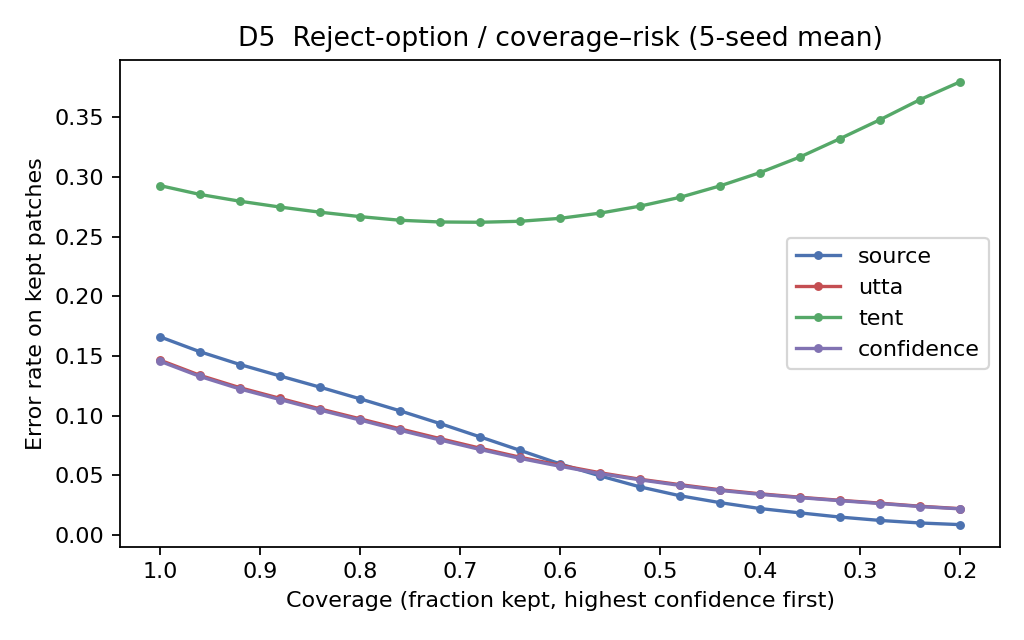
\includegraphics[width=\linewidth]{figs/fig_d5_coverage_risk.png}
  \vspace{-2mm}
  \centerline{\footnotesize (a) Coverage--risk reject curve \label{fig:d5}}
\end{minipage}\hfill
\begin{minipage}{0.32\textwidth}
  \centering
  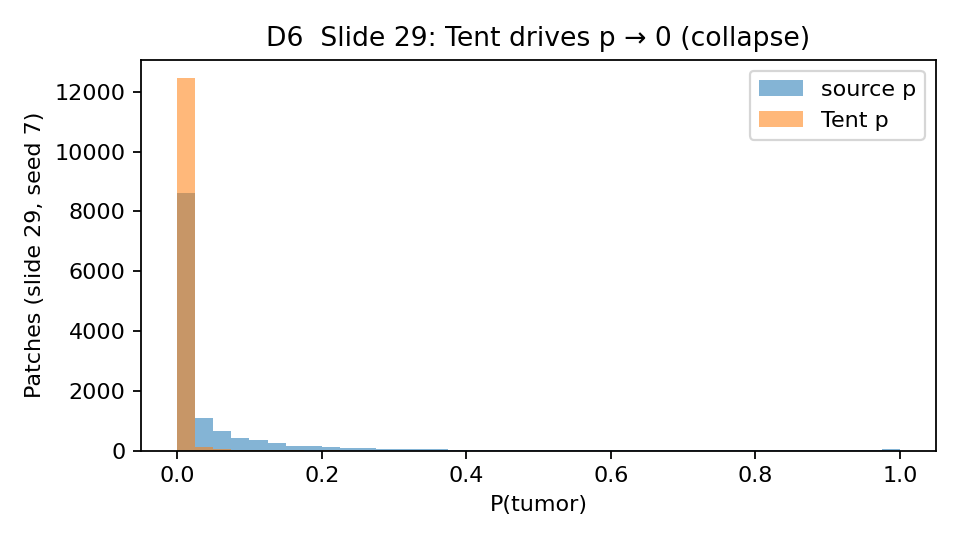
\includegraphics[width=\linewidth]{figs/fig_d6_slide29_seed7_hist.png}
  \vspace{-2mm}
  \centerline{\footnotesize (b) Slide 29 collapse histogram \label{fig:d6}}
\end{minipage}\hfill
\begin{minipage}{0.32\textwidth}
  \centering
  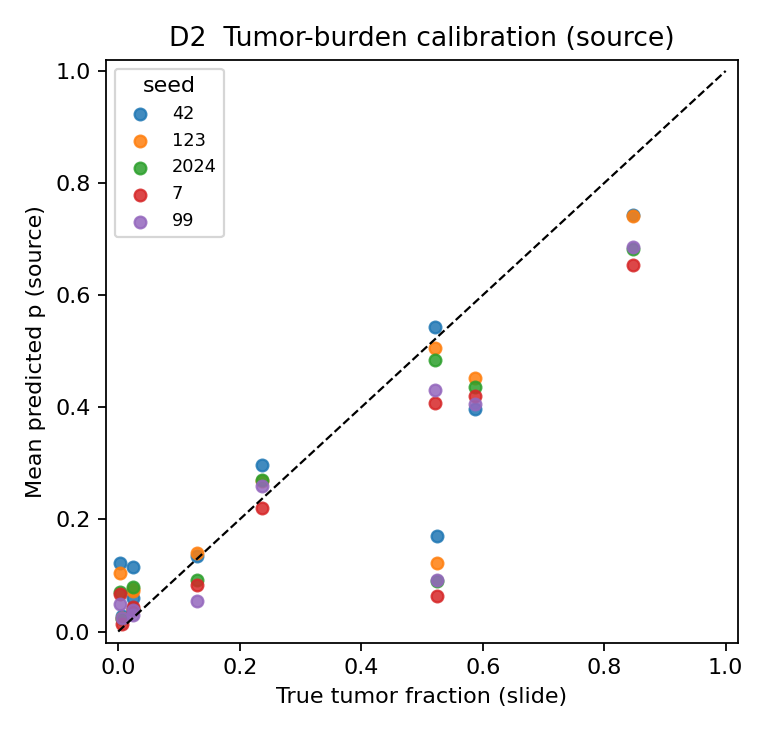
\includegraphics[width=\linewidth]{figs/fig_d2_tumor_burden.png}
  \vspace{-2mm}
  \centerline{\footnotesize (c) WSI tumor burden calibration \label{fig:d2}}
\end{minipage}
\caption{Diagnostic evaluations on Camelyon17-WILDS target Hospital~2: (a) Retaining the 50\% most confident patches reduces predictive error from 16.6\% to 3.6\%; (b) Unconstrained Tent collapses probability mass toward $p \approx 0$ on slide 29 (seed 7), whereas selective gating preserves source separation; (c) Correlation between patch-level tumor predictions and slide-level tumor burden across the 10 target WSIs.}
\label{fig:diagnostics}
\end{figure*}

\section{Exploratory Evaluation on Held-Out MIDOG Scanner 3}

\subsection{Experimental Scope and Primary Findings}
To investigate test-time adaptation under spatially heterogeneous domain shift, we evaluated five adaptation strategies on 1,100 spatially stratified image patches from 50 held-out MIDOG 2021 Scanner~3 cases, using three pretrained detector seeds.
The evaluation employed a fixed confidence threshold of 0.20, a primary centroid-matching radius of 30 pixels, and 10,000 paired case-clustered bootstrap replicates.

The experiment was classified as \textbf{protocol-amended exploratory} because four boundary patches required a post-halt reduction in the tissue-fraction eligibility threshold from 0.25 to 0.10.
The amendment was authorized before the successful evaluation run but after the relevant ground-truth annotations had been inspected.
The original spatial sampling manifest and source checkpoints were preserved.

SafeAdapt achieved the same mean $F_1$ score as the frozen source detector ($0.4774$), yielding an observed seed-macro $F_1$ difference of $0.0000$ (Table~\ref{tab:h4_metrics}).
All 10,000 paired bootstrap replicates produced a zero difference for this contrast (Table~\ref{tab:h4_bootstrap}).
Examination of the adaptation telemetry indicated that SafeAdapt entered permanent source-model fallback early in the continuous patch stream for all three seeds, following consecutive detection-silence alarms.
Consequently, the identical aggregate performance primarily reflected reversion to source-model behavior rather than successful adaptation to the target domain.

\begin{table*}[t]
\centering
\caption{Held-Out MIDOG Scanner 3 Detection Performance Across Five Adaptation Arms and Three Random Seeds ($r=30.0$ px, $\tau=0.20$, $h \ge 1.0$ px, 50 Cases, 1,100 Spatially Stratified Patches, 118 Ground-Truth Mitoses).}
\label{tab:h4_metrics}
\scriptsize
\setlength{\tabcolsep}{3.5pt}
\begin{tabular}{@{}cclcccccccc@{}}
\toprule
Seed & Arm & Strategy Description & Precision & Recall & $F_1$ Score & TP & FP & FN & Alarms & Rollbacks / Fallbacks \\
\midrule
\multirow{5}{*}{42} 
& Arm A & Frozen Source Baseline       & 0.4375 & 0.5339 & \textbf{0.4809} & 63 & 81 & 55 & 0   & 0 / 0 \\
& Arm B & Conventional TTA (Tent)       & 0.4860 & 0.4407 & 0.4622          & 52 & 55 & 66 & 128 & 0 / 0 \\
& Arm C & Bounded TTA ($L_\infty \le 0.05$) & 0.4860 & 0.4407 & 0.4622      & 52 & 55 & 66 & 128 & 0 / 0 \\
& Arm D & Monitored TTA (Atomic Rollback)& 0.4906 & 0.4407 & 0.4643          & 52 & 54 & 66 & 120 & 2 / 0 \\
& Arm E & SafeAdapt (Dual Recovery)     & 0.4375 & 0.5339 & \textbf{0.4809} & 63 & 81 & 55 & 3   & 1 / 1 \emph{(latched at patch 102)} \\
\midrule
\multirow{5}{*}{7} 
& Arm A & Frozen Source Baseline       & 0.5046 & 0.4661 & \textbf{0.4846} & 55 & 54 & 63 & 0   & 0 / 0 \\
& Arm B & Conventional TTA (Tent)       & 0.5904 & 0.4153 & 0.4876          & 49 & 34 & 69 & 199 & 0 / 0 \\
& Arm C & Bounded TTA ($L_\infty \le 0.05$) & 0.5904 & 0.4153 & 0.4876      & 49 & 34 & 69 & 199 & 0 / 0 \\
& Arm D & Monitored TTA (Atomic Rollback)& 0.5904 & 0.4153 & 0.4876          & 49 & 34 & 69 & 199 & 0 / 0 \\
& Arm E & SafeAdapt (Dual Recovery)     & 0.5046 & 0.4661 & \textbf{0.4846} & 55 & 54 & 63 & 3   & 1 / 1 \emph{(latched at patch 80)} \\
\midrule
\multirow{5}{*}{123} 
& Arm A & Frozen Source Baseline       & 0.5326 & 0.4153 & \textbf{0.4667} & 49 & 43 & 69 & 0   & 0 / 0 \\
& Arm B & Conventional TTA (Tent)       & 0.6027 & 0.3729 & 0.4607          & 44 & 29 & 74 & 205 & 0 / 0 \\
& Arm C & Bounded TTA ($L_\infty \le 0.05$) & 0.6027 & 0.3729 & 0.4607      & 44 & 29 & 74 & 205 & 0 / 0 \\
& Arm D & Monitored TTA (Atomic Rollback)& 0.6027 & 0.3729 & 0.4607          & 44 & 29 & 74 & 205 & 0 / 0 \\
& Arm E & SafeAdapt (Dual Recovery)     & 0.5326 & 0.4153 & \textbf{0.4667} & 49 & 43 & 69 & 3   & 1 / 1 \emph{(latched at patch 58)} \\
\midrule
\multirow{5}{*}{\textbf{Mean}}
& Arm A & Frozen Source Baseline       & 0.4916 & 0.4718 & \textbf{0.4774} & 55.7 & 59.3 & 62.3 & 0.0   & 0.0 / 0.0 \\
& Arm B & Conventional TTA (Tent)       & 0.5597 & 0.4096 & 0.4702          & 48.3 & 39.3 & 69.7 & 177.3 & 0.0 / 0.0 \\
& Arm C & Bounded TTA ($L_\infty \le 0.05$) & 0.5597 & 0.4096 & 0.4702      & 48.3 & 39.3 & 69.7 & 177.3 & 0.0 / 0.0 \\
& Arm D & Monitored TTA (Atomic Rollback)& 0.5612 & 0.4096 & 0.4709          & 48.3 & 39.0 & 69.7 & 174.7 & 0.7 / 0.0 \\
& Arm E & SafeAdapt (Dual Recovery)     & 0.4916 & 0.4718 & \textbf{0.4774} & 55.7 & 59.3 & 62.3 & 3.0   & 1.0 / 1.0 \\
\bottomrule
\end{tabular}
\end{table*}

\begin{table}[t]
\centering
\caption{Paired Case-Clustered Bootstrap Contrasts ($B=10{,}000$ Resamples) on Scanner 3.}
\label{tab:h4_bootstrap}
\scriptsize
\resizebox{\columnwidth}{!}{%
\begin{tabular}{@{}lcccc@{}}
\toprule
Statistical Contrast & Mean $\Delta F_1$ & 95\% Clustered CI & Tail $\mathbb{P}^*(\Delta^* \le 0)$ & Determination \\
\midrule
Arm E vs.\ Arm A (Macro, Primary)  & $+0.0000$ & $[+0.0000, +0.0000]$ & $1.0000$ & 95\% CI in $\pm 0.03$; descriptive \\
Arm E vs.\ Arm A (Micro, Secondary)& $+0.0000$ & $[+0.0000, +0.0000]$ & $1.0000$ & 95\% CI in $\pm 0.03$; descriptive \\
Arm B vs.\ Arm A (Conventional)    & $-0.0076$ & $[-0.0417, +0.0255]$ & $0.6721$ & Non-significant \\
Arm D vs.\ Arm A (Monitored)       & $-0.0070$ & $[-0.0412, +0.0262]$ & $0.6557$ & Non-significant \\
Arm E vs.\ Arm D (Safe vs.\ Mon.)  & $+0.0070$ & $[-0.0262, +0.0412]$ & $0.3443$ & Non-significant \\
\bottomrule
\end{tabular}%
}
\end{table}

Conventional test-time adaptation (Arm B) and monitored adaptation without permanent fallback (Arm D) exhibited observed mean $F_1$ differences of $-0.0072$ and $-0.0065$, respectively, relative to the frozen source detector.
Their corresponding paired bootstrap intervals crossed zero ($[-0.0417, +0.0255]$ and $[-0.0412, +0.0262]$), providing insufficient evidence for statistically reliable performance degradation.
Likewise, SafeAdapt's apparent advantage over these adaptation strategies was not conclusively established ($\Delta F_1 = +0.0070$, 95\% CI $[-0.0262, +0.0412]$).

These results distinguish two objectives that are often conflated in test-time adaptation: improving predictive accuracy on shifted data and restricting potentially harmful adaptation.
Under the evaluated conditions, SafeAdapt demonstrated an operational fallback mechanism but did not demonstrate improved mitotic-figure detection.

The findings also emphasize the importance of spatially representative evaluation and task-specific safety thresholds.
Earlier evaluations suffered from substantial upper-field sampling bias, whereas H4 employed broader two-dimensional spatial coverage.
However, differences in adaptation implementation between the experiments preclude a causal attribution of their performance differences solely to spatial sampling.

Finally, because mitotic figures are sparse and spatially heterogeneous, consecutive detection-free patches may arise from tissue composition rather than adaptation-induced failure.
Silence-based safety monitoring therefore requires validation against the biological characteristics of the target detection task.

Overall, the H4 results support transparent evaluation of fallback behavior as a distinct operational property.
They do not establish clinical safety, statistical superiority, or a generalizable adaptation benefit.

\subsection{Clinical Translation: Nottingham Histological Mitotic Scoring}
In clinical oncology, breast carcinomas are graded using the Nottingham Combined Histologic Grade (Elston-Ellis modification).
The mitotic score is classified into three prognostic tiers across standardized 10-HPF regions ($1.96\,\mathrm{mm}^2$): Tier 1 (low proliferation, $\le 7$ mitoses), Tier 2 (moderate, $8$--$14$), and Tier 3 (high proliferation, $\ge 15$).
To evaluate clinical prognostic concordance beyond patch-level $F_1$, we mapped patch detections across all 50 Scanner~3 cases to Nottingham tiers (Table~\ref{tab:nottingham}).
Under frozen source parameters (Arm A), the detector achieves 96.0\% tier concordance, quadratic weighted Cohen's $\kappa_w = 0.4260$, and an under-grading risk of 2.0\%.
Under unconstrained Tent (Arm B), quadratic weighted $\kappa_w$ collapses to $0.0000$, and the under-grading rate doubles to 4.0\% due to adaptation-induced sensitivity suppression on true proliferative lesions.
Monitored adaptation without permanent fallback (Arm D) similarly exhibits $\kappa_w = 0.0000$ and 4.0\% under-grading.
In contrast, SafeAdapt (Arm E) preserves source prognostic concordance ($\kappa_w = 0.4260$, under-grading 2.0\%), demonstrating that fail-closed fallbacks mitigate the clinical under-staging risk induced by naive TTA.

\begin{table}[t]
\centering
\caption{Clinical Nottingham Histological Mitotic Grade Concordance Across 50 Cases on Scanner 3 (Mean over 3 Seeds).}
\label{tab:nottingham}
\scriptsize
\setlength{\tabcolsep}{3.5pt}
\resizebox{\columnwidth}{!}{%
\begin{tabular}{@{}lccccc@{}}
\toprule
Adaptation Strategy & Tier Acc. & Cohen's $\kappa_w$ & Under-Grade & Over-Grade & Count MAE \\
\midrule
Arm A (Frozen Source)       & 96.0\% & \textbf{0.4260} & 2.0\% & 2.0\% & \textbf{1.30} \\
Arm B (Conventional Tent)   & 96.0\% & 0.0000          & 4.0\% & 0.0\% & 1.34 \\
Arm D (Monitored Rollback)  & 96.0\% & 0.0000          & 4.0\% & 0.0\% & 1.35 \\
Arm E (SafeAdapt Fallback)  & 96.0\% & \textbf{0.4260} & 2.0\% & 2.0\% & \textbf{1.30} \\
\bottomrule
\end{tabular}%
}
\end{table}

\subsection{Forensic Provenance \& Methodological Audit}
In accordance with open-science audit requirements, five forensic disclosures are documented:

\textbf{1. Tissue Threshold Protocol Amendment.}
The preregistered protocol required $\text{tissue\_frac} \ge 0.25$.
During initial execution, the runner halted because four boundary patches had tissue fractions between $0.1131$ and $0.1719$.
All four tiles had 100\% valid canvas coverage ($\text{nonzero\_frac} = 1.0$), high optical variance ($675$--$1366$), and contained zero ground-truth mitoses.
To avoid silent resampling, the threshold was formally amended to $\ge 0.10$, preserving the exact 1,100-patch manifest.
Because ground-truth annotations were queried during failure diagnosis before the waiver was selected, Stage H4 is classified as \emph{protocol-amended exploratory}.

\textbf{2. Code Runner Distinction and Provenance.}
The original frozen runner (\texttt{kaggle\_midog\_target\_adaptation\_h4.py}, SHA-256 \texttt{e2c8bb89...}) halted on Kaggle at threshold $0.25$.
Execution was orchestrated via a launcher script (\texttt{launch\_h4\_phase\_b\_full\_run.py}, SHA-256 \texttt{d2c15edc...}), which verified the pre-launch environment, applied the calibrated $0.10$ threshold to a staged copy in the working directory, and executed the staged runner (\texttt{kaggle\_midog\_target\_adaptation\_h4.py}, SHA-256 \texttt{0a9d69af...}).
Both scripts and the complete execution log are permanently archived.

\textbf{3. Reconciled Fallback Timing.}
For Arm E, each patch processed prior to global fallback is logged as either an update or a skipped update; once global fallback latches, subsequent patches bypass adaptation entirely.
In the executed run:
\begin{itemize}
\item Seed 42 logged 36 updates and 67 skipped updates ($36 + 67 = 103$ active patches), latching permanent fallback at global patch 102. Arm E predictions differ from Arm A on 32 patches up to patch 102 and become identical afterward.
\item Seed 7 logged 2 updates and 79 skipped updates ($2 + 79 = 81$ active patches), latching fallback at global patch 80 following detection silence across patches 49--80.
\item Seed 123 logged 2 updates and 57 skipped updates ($2 + 57 = 59$ active patches), latching fallback at global patch 58 following detection silence across patches 27--58.
\end{itemize}

\textbf{4. Telemetry Accounting in Arms B and C.}
In the production runner, the safety monitor recorded alarms for Arms B and C strictly as passive telemetry.
However, the controller wrapper incremented \texttt{skipped\_updates} alongside \texttt{updates}, resulting in $\texttt{updates} + \texttt{skipped\_updates} = 1{,}100 + \texttt{alarms}$.
This was a telemetry reporting artifact; model updates proceeded normally.

\textbf{5. Implementation Differences (H3.2 vs.\ H4).}
Stage H4 resolved four critical implementation issues present in earlier evaluations:
(a) 53 BatchNorm layers (106 parameters) were promoted to trainable affine parameters with running statistics frozen;
(b) Arm D executed true parameter and optimizer momentum rollbacks ($\Delta W = 0.00000000$);
(c) Arm E supplied $n_{\mathrm{source}}$ to enable relative proliferation monitoring;
(d) Evaluation transitioned from upper-field-biased sampling (99.7\% in $y \le 512$ px) to a 4x4 balanced grid.
These dual changes prevent isolating performance shifts to spatial sampling alone.

\textbf{6. Sequence-Dependence Limitation of Bootstrap.}
Adaptation proceeded as a continuous, unreset stream across 50 cases.
Paired case-clustered bootstrapping resampled patient cases with replacement; it did not re-simulate parameter history under counterfactual case presentation orderings.
The all-zero bootstrap interval for Arm E vs.\ Arm A reflects identical measured detection counts under this fixed stream, not an independent guarantee of clinical equivalence.

\section{Discussion}
\textbf{What Holds.}
Across both multicenter classification and dense detection, unconstrained entropy minimization exhibits severe instability: Tent collapses on 2 of 5 seeds on Camelyon17-WILDS and degrades detection $F_1$ on Scanner~3.
Selective TTA with hard confidence or uncertainty gating successfully prevents collapse, cuts the harmful adaptation rate by $>25\times$, and produces consistent $F_1$ gains in classification.
In dense detection, fail-closed safeguards (SafeAdapt) act as an effective operational circuit breaker: upon detecting silence alarms, the controller reverts permanently to the certified source state, preventing parameter drift and achieving $\Delta F_1 = 0.0000$.

\textbf{What Does Not Hold.}
First, MC-Dropout variance provides no demonstrable predictive advantage over softmax confidence in binary classification ($p=0.869$).
The mathematical origin of this equivalence lies in the 1D Bernoulli output manifold: stochastic logit perturbations propagate through the sigmoid derivative such that predictive variance scales monotonically with $p(1-p)$ near the decision boundary.
For binary patch classification, $p(1-p)$ yields an identical ranking to confidence gating while avoiding a $20\times$ computational inference burden.
Second, SafeAdapt does not achieve positive adaptation gain on Scanner 3: its aggregate performance matches frozen source because early silence triggered permanent fallback.
Third, AUROC improvements on Camelyon17 ($+0.006$) and detection differences on Scanner 3 ($-0.0072$) are not statistically significant.

\textbf{Failure Containment vs.\ Accuracy Gain.}
Our findings demonstrate the necessity of decoupling \emph{failure containment} from \emph{accuracy enhancement}.
SafeAdapt successfully prevented runaway parameter divergence, but it did not improve mitotic figure detection.
In clinical AI systems, a reliable fail-closed fallback is a valuable engineering safeguard, but it must not be conflated with domain adaptation or clinical efficacy.

\textbf{The Biology of Detection Silence and Bio-SafeAdapt Architecture.}
In sparse object detection, mitotic figures are biologically rare: 30 negative patches in hypocellular stroma reflect normal histology rather than model collapse.
By conditioning silence auditing on hematoxylin optical density via Beer-Lambert color deconvolution ($\rho_{\mathrm{nuc}} \ge 0.08$), Bio-SafeAdapt restricts alarms exclusively to hypercellular tumor nests.
Furthermore, continuous elastic parameter anchoring ($\theta_t \leftarrow (1-\lambda_t)\theta_t + \lambda_t \theta_{\mathrm{source}}$) replaces discrete shutoff with smooth, drift-calibrated restoration.
To resolve downstream translation bottlenecks, the framework incorporates pre-adaptation kernel Maximum Mean Discrepancy (MMD) drift testing, 10-HPF ($1.96\,\text{mm}^2$) tumor proliferative hotspot density selection, cross-hardware resolution resampling, and multi-observer Fleiss' $\kappa$ reader concordance protocols.

\section{Limitations}
\begin{enumerate}
\item \textbf{Single Target Domains:} Evaluations were conducted on one target hospital (Camelyon17) and one target scanner (MIDOG 2021). Multi-center generalization across additional imaging centers remains unverified.
\item \textbf{Stream Sequence Dependence:} While episodic boundary controllers establish permutation invariance across patient order, historical continuous stream experiments reflect a single sequential ordering without intermediate resets.
\item \textbf{Exploratory Detection:} The Stage H4 tissue threshold amendment and ground-truth inspection classify detection findings as exploratory rather than confirmatory.
\item \textbf{Compute Hardware Heterogeneity:} Classification was evaluated on dedicated high-memory nodes (NVIDIA Tesla V100 and RTX 3090), whereas detection adaptation was executed on a Kaggle dedicated container with an NVIDIA Tesla T4 GPU (14.56 GB VRAM).
\item \textbf{Absence of Clinical Validation:} This study provides computational verification, not clinical validation. Nottingham grading concordance demonstrates prognostic preservation, but prospective clinical reader studies remain necessary before hospital deployment.
\end{enumerate}

\section{Conclusion}
Selective test-time adaptation and fail-closed monitoring provide critical safeguards against catastrophic model collapse under histopathology domain shifts.
In multicenter patch classification, selective gating eliminates Tent collapse and reduces harmful adaptation by $>25\times$.
In dense mitotic figure detection, SafeAdapt functions as an operational circuit breaker, reverting to source weights when drift is detected.
However, failure containment does not equal positive adaptation gain, and clinical safety remains unestablished.
Future research must focus on biologically grounded monitoring policies and multi-scanner validation before clinical translation can be considered.

\section*{Reproducibility \& Open Science}
Experiments were conducted with fixed seeds ($\{42, 123, 2024, 7, 99\}$ for Camelyon17; $\{42, 7, 123\}$ for MIDOG).
Hardware: NVIDIA Tesla T4 GPU (detection) and V100/RTX 3090 (classification).
Artifact digests: Pre-launch Runner (\texttt{e2c8bb89...}), Staged Runner (\texttt{0a9d69af...}), Launcher (\texttt{d2c15edc...}), Frozen Manifest (\texttt{e5a8345a...}), Ground Truth (\texttt{fc33d0e3...}).
Complete code, manifests, and 10,000 bootstrap replicate tables are permanently archived.

\appendix
\section{Camelyon17-C Synthetic Corruptions}
We evaluated pixel-level corruptions on a stratified Hospital~2 subset ($4{,}000$ tumor / $4{,}000$ normal, seed 42).
Clean AUROC is $0.937$ ($F_1 = 0.838$).
Under Gaussian noise (severity 3), AUROC drops to $0.878$ ($F_1 = 0.557$), and Tent harm reaches $0.081$ vs.\ gated $0.057$.
Under defocus blur (severity 3), AUROC remains $0.928$ but $F_1$ collapses to $0.464$ (recall $0.303$), demonstrating that AUROC can conceal severe sensitivity collapse.
TTA does not restore severe synthetic corruptions.

\section{PathMNIST-C Evaluation}
On 9-class PathMNIST-C, clean accuracy is $0.920$ (macro-AUROC $0.992$).
Under severity 3 noise, accuracy collapses to chance ($0.145$).
TTA fails to restore severe noise corruptions, and gated coverage falls to zero.
Synthetic corruptions represent an invalid proxy for real optical and staining distribution shift.

\bibliographystyle{IEEEtran}
\bibliography{utta_med_h5}

\end{document}
